\documentclass[11pt]{article}
\usepackage{geometry}                % See geometry.pdf to learn the layout options. There are lots.
\geometry{a4paper}                   % ... or a4paper or a5paper or ... 
%\geometry{landscape}                % Activate for for rotated page geometry
%\usepackage[parfill]{parskip}    % Activate to begin paragraphs with an empty line rather than an indent
\usepackage[utf8]{inputenc}
\usepackage{newunicodechar}
\usepackage{graphicx}
\usepackage{amssymb}
\usepackage{epstopdf}
\usepackage{listings}
\usepackage{longtable}
\usepackage{colortbl}
\usepackage[table]{xcolor}
\usepackage{underscore}
\usepackage{xcolor}
\usepackage{tikzpagenodes}
\usepackage{eso-pic}

\usetikzlibrary{calc}
\usetikzlibrary{positioning}
\usepgflibrary{shapes.geometric}
\usetikzlibrary{shapes.misc}
\usetikzlibrary{arrows}

%\AddToShipoutPictureBG{%
%\begin{tikzpicture}[overlay,remember picture]
%\draw[line width=0.5pt]
%      ($ (current page text area.north west) $)
%      rectangle
%      ($ (current page text area.south east) $);
%\end{tikzpicture}
%}

\makeatletter
\newcommand*{\pmzeroslash}{%
  \nfss@text{%
    \sbox0{0}%
    \sbox2{/}%
    \sbox4{%
      \raise\dimexpr((\ht0-\dp0)-(\ht2-\dp2))/2\relax\copy2 %
    }%
    \ooalign{%
      \hfill\copy4 \hfill\cr
      \hfill0\hfill\cr
    }%
    \vphantom{0\copy4 }% correct overall height and depth of the symbol
  }%
}
\makeatother



\definecolor{seagreen}{RGB}{64,100,120}
\definecolor{darkpink}{RGB}{200,100,120}
\definecolor{light-gray}{gray}{0.85}
\definecolor{medium-gray}{gray}{0.5}

\DeclareGraphicsRule{.tif}{png}{.png}{`convert #1 `dirname #1`/`basename #1 .tif`.png}

\lstdefinelanguage{goilTemplate}
{
  morekeywords= {
	  after,
	  before,
	  between,
	  default,
	  do,
	  down,
	  up,
	  else,
	  elsif,
	  emptylist,
	  emptymap,
	  end,
	  error,
	  exists,
	  false,
	  for,
	  foreach,
	  from,
	  here,
	  unlet,
	  let,
	  loop,
	  no,
	  if,
	  in,
	  mod,
	  not,
	  or,
	  step,
	  template,
	  then,
	  to,
	  true,
	  yes,
	  warning,
	  while,
	  write,
	  display,
	  print,
	  println,
	  repeat,
	  !,
	  ?
	}
}

\lstset{
  language=goilTemplate,
  emph={
    condition,
    var,
    variable,
    expression,
    expression_start,
    expression_end,
    increment,
    string,
    instruction_list,
    instruction_list_1,
    instruction_list_2,
    template_file_name,
    getter,
    setter,
    hierarchy,
    index,
    key,
    limit_expression
  },
  emphstyle=\em,
  moredelim=[s][\color{blue}]{\%}{\%},
  moredelim=[s]{"}{"},
  morecomment=[l][\color{medium-gray}\itshape]{\#},
  basicstyle=\ttfamily\small,
  morekeywords=\bfseries,
  frame=tb,
}

\newcommand{\character}[1]{{\small\ttfamily `{#1}'}}

\newcommand{\argu}[1]{{\ttfamily #1}}
\newcommand{\ctype}[1]{{\small\ttfamily #1}}
\newcommand{\cdata}[1]{{\ttfamily #1}}
\newcommand{\var}[1]{{\small\ttfamily #1}}
\newcommand{\va}{\small\ttfamily\em}
\newcommand{\cfunction}[1]{{\ttfamily #1}}
\newcommand{\cmacro}[1]{{\small\ttfamily #1}}
\newcommand{\constant}[1]{{\small\ttfamily #1}}
\newcommand{\oilobj}[1]{{\small\ttfamily #1}}
\newcommand{\oilattr}[1]{{\small\ttfamily #1}}
\newcommand{\oilval}[1]{{\small\ttfamily #1}}
\newcommand{\member}[1]{{\small\ttfamily #1}}
\newcommand{\mem}{\small\ttfamily}
\newcommand{\tool}[1]{{\em #1}}
\newcommand{\na}{\scriptsize\ttfamily NA}

\renewcommand{\ttdefault}{pcr}

\newcommand\Warning{%
 \makebox[1.4em][c]{%
 \makebox[0pt][c]{\raisebox{-.05em}{\scriptsize!}}%
 \makebox[0pt][c]{\raisebox{-.2em}{\color{red}\Large$\bigtriangleup$}}}}%

\newcommand{\warning}[1]{%
\vspace{1em}
\hspace{-18.3mm}
\rowcolors{1}{white}{light-gray}
\begin{tabular}[b]{m{5mm}|m{\linewidth}}
\Warning & #1\\
\end{tabular}
}


\title{GTL Template language}
\author{Jean-Luc B\'echennec}
%\date{}                                           % Activate to display a given date or no date

\begin{document}
\maketitle
%\section{}
%\subsection{}

\tableofcontents

\newpage
\section{Data types}

GTL supports the following data types:
\begin{description}
\item[int] arbitrary precision integer numbers. The GMP library is used;
\item[float] 64 bits floating point numbers;
\item[bool] standard boolean;
\item[type] the type of a data;
\item[string] unicode strings;
\item[struct] structured data;
\item[list] lists of data, may be accessed as a table;
\item[map] map (aka dictionary) of data;
\item[unconstructed] an unconstructed variable.
\end{description}

Each type has its set of operators, getters and setters. The expression, for getters, or the variable, for setters, is called the {\em target}. Getters return a value related to the data but do not change it. They are used to get information from a data or to convert it into another type. Setter may target a literal expressions. Setters change the data and do not return anything. Setter may only target a variable. Getters and setters may have arguments. Syntax for getters without argument is as follow:

\begin{lstlisting}[language=goilTemplate]
[expression getter]
\end{lstlisting}

When the getter takes arguments, they are listed after a colon and separated commas as follow:

\begin{lstlisting}[language=goilTemplate]
[expression getter : arg1, arg2, ..., argN]
\end{lstlisting}

Syntax for setters without arguments is as follow:

\begin{lstlisting}[language=goilTemplate]
[!variable setter]
\end{lstlisting}

When the setter takes arguments, they are listed after a colon and separated by commas as follow:

\begin{lstlisting}[language=goilTemplate]
[!variable setter : arg1, arg2, ..., argN]
\end{lstlisting}

\subsection{getters applicable to any data type}

\paragraph{\lstinline{type}} returns the data type of the expression. See the section \ref{sec:type}.

\paragraph{\lstinline{isANumber}} returns \lstinline{true} if the expression is a number: \lstinline{int} or \lstinline{float}, \lstinline{false} otherwise.

\subsection{\lstinline{int} data type}

The \lstinline{int} data type support arbitrary precision arithmetic by using the GNU Multiple Precision Arithmetic Library (GMP).

\subsubsection{\lstinline{int} operators}

The \lstinline{int} datatype supports the following operators:

\paragraph{Unary operators}~

\rowcolors{1}{white}{light-gray}
\begin{longtable}{>{\ttfamily}l|>{\ttfamily}l|p{3.34in}}
{\bf Operator}&{\bf Expression type}&{\bf Meaning}\\
\hline\endhead
 {+}&
  {int $\leftarrow$ +int}&
  {Plus operator. No effect}\\
 {-}&
  {int $\leftarrow$ -int}&
  {Minus operator. Negation}\\
 {\raisebox{-1.2mm}{\textasciitilde}}&
  {int $\leftarrow$ \raisebox{-1.2mm}{\textasciitilde}int}&
  {Not operator. Complementation by 1}\\
\end{longtable}

\paragraph{Binary arithmetic operators}~

\rowcolors{1}{white}{light-gray}
\begin{longtable}{>{\ttfamily}l|>{\ttfamily}l|p{3.14in}}
{\bf Operator}&{\bf Expression type}&{\bf Meaning}\\
\hline\endhead
 {+}&
  {int $\leftarrow$ int + int}&
  {Addition}\\
 {-}&
  {int $\leftarrow$ int - int}&
  {Substraction}\\
 {*}&
  {int $\leftarrow$ int * int}&
  {Multiplication}\\
 {/}&
  {int $\leftarrow$ int / int}&
  {Division}\\
 {mod}&
  {int $\leftarrow$ int mod int}&
  {Modulus}\\
\end{longtable}

\paragraph{Binary bitwise operators}~

\rowcolors{1}{white}{light-gray}
\begin{longtable}{>{\ttfamily}l|>{\ttfamily}l|p{3.22in}}
{\bf Operator}&{\bf Expression type}&{\bf Meaning}\\
\hline\endhead
 {\&}&
  {int $\leftarrow$ int \& int}&
  {bitwise and}\\
 {|}&
  {int $\leftarrow$ int \rule{1pt}{1.5ex} int}&
  {bitwise or}\\
 {\^~}&
  {int $\leftarrow$ int \^{} int}&
  {bitwise exclusive or}\\
 {<<}&
  {int $\leftarrow$ int << int}&
  {shift left}\\
 {>>}&
  {int $\leftarrow$ int >> int}&
  {shift right}\\
\end{longtable}

\paragraph{Comparison operators}~

\rowcolors{1}{white}{light-gray}
\begin{longtable}{>{\ttfamily}l|>{\ttfamily}l|p{3.15in}}
{\bf Operator}&{\bf Expression type}&{\bf Meaning}\\
\hline\endhead
 {!=}&
  {bool $\leftarrow$ int != int}&
  {Not equal}\\
 {==}&
  {bool $\leftarrow$ int == int}&
  {Equal}\\
 {>}&
  {bool $\leftarrow$ int > int}&
  {Greater than}\\
 {<}&
  {bool $\leftarrow$ int < int}&
  {Lower than}\\
 {>=}&
  {bool $\leftarrow$ int >= int}&
  {Greater or equal}\\
 {<=}&
  {bool $\leftarrow$ int <= int}&
  {Lower or equal}\\
\end{longtable}

\subsubsection{\lstinline{int} getters}

\rowcolors{1}{white}{light-gray}
\begin{longtable}{>{\ttfamily}l|l|p{3.13in}}
{\bf getter}&{\bf Type}&{\bf Meaning}\\
\hline\endhead
 {string}&
  {string}&
  {Returns a string decimal representation of the int expression. \texttt{[42 string]} returns string \texttt{"42"}.}\\
 {hexString}&
  {string}&
  {Returns a string hexadecimal representation of the int expression prefixed by \texttt{0x}. If the expression is negative a `-' is inserted before. \texttt{[42 hexString]} returns string \texttt{"0x2A"}. \texttt{[-1 hexString]} returns string \texttt{"-0x1"}.}\\
 {xString}&
  {string}&
  {Returns a string hexadecimal representation of the int expression. If the expression is negative a `-' is inserted before. \texttt{[42 xString]} returns string \texttt{"2A"}. \texttt{[-42 xString]} returns string \texttt{"-2A"}.}\\
 {numberOfBytes}&
  {int}&
  {Returns the number of bytes needed to store an unsigned expression. \texttt{[255 numberOfBytes]} returns \texttt{1}, \texttt{[256 numberOfBytes]} returns \texttt{2}}\\
 {signedNumberOfBytes}&
  {int}&
  {Returns the number of bytes needed to store a signed expression. \texttt{[127 numberOfBytes]} returns \texttt{1}, \texttt{[128 numberOfBytes]} returns \texttt{2}}\\
 {numberOfBits}&
  {int}&
  {Returns the number of bits needed to store an unsigned expression. \texttt{[63 numberOfBits]} returns \texttt{6}, \texttt{[64 numberOfBits]} returns \texttt{7}}\\
 {signedNumberOfBits}&
  {int}&
  {Returns the number of bits needed to store a signed expression. \texttt{[63 signedNumberOfBits]} returns \texttt{7}, \texttt{[64 signedNumberOfBits]} returns \texttt{8}}\\
 {sign}&
  {int}&
  {Returns \texttt{-1} if the expression is strictly negative, \texttt{0} if it is null and \texttt{+1} if the expression is strictly positive.}\\
 {fitsUnsignedInByte}&
  {bool}&
  {Returns \texttt{true} if the expression fits in an unsigned byte, \texttt{false} otherwise.}\\
 {fitsSignedInByte}&
  {bool}&
  {Returns \texttt{true} if the expression fits in a signed byte, \texttt{false} otherwise.}\\
 {fitsUnsignedInWord}&
  {bool}&
  {Returns \texttt{true} if the expression fits in an unsigned 16 bits word, \texttt{false} otherwise.}\\
 {fitsSignedInWord}&
  {bool}&
  {Returns \texttt{true} if the expression fits in a signed 16 bits word, \texttt{false} otherwise.}\\
 {fitsUnsignedInLong}&
  {bool}&
  {Returns \texttt{true} if the expression fits in an unsigned 32 bits long, \texttt{false} otherwise.}\\
 {fitsSignedInLong}&
  {bool}&
  {Returns \texttt{true} if the expression fits in a signed 32 bits long, \texttt{false} otherwise.}\\
 {fitsUnsignedInLongLong}&
  {bool}&
  {Returns \texttt{true} if the expression fits in an unsigned 64 bits long long, \texttt{false} otherwise.}\\
 {fitsSignedInLongLong}&
  {bool}&
  {Returns \texttt{true} if the expression fits in a signed 64 bits long long, \texttt{false} otherwise.}\\
 {abs}&
  {int}&
  {Returns the absolute value of the expression.}\\
 {bitAtIndex}&
  {bool}&
  {This getter takes one argument: \texttt{index}. It returns \texttt{true} if the bit at index \texttt{index} is set and \texttt{false} otherwise. \texttt{index} 0 corresponds to the lowest significant bit. \texttt{[1 bitAtIndex: 0]} returns \texttt{true}}\\
\end{longtable}

\subsubsection{\lstinline{int} setters}

\rowcolors{1}{white}{light-gray}
\begin{longtable}{>{\ttfamily}l|p{3.84in}}
{\bf setter}&{\bf Meaning}\\
\hline\endhead
 {setBitAtIndex}&
  {This setter takes two arguments. The first one, \texttt{value}, is a bool. The second one, \texttt{index}, is the index of the bit to set. if \texttt{value} is \texttt{true} the bit is set to \texttt{1} and to \texttt{0} otherwise. Assuming \texttt{a} contains \texttt{0} at start, \texttt{[!a setBitAtIndex: true, 0]} sets \texttt{a} to \texttt{1}.}\\
 {complementBitAtIndex}&
  {This setter takes one argument, \texttt{index}, which is the index of the bit to complement.  Assuming \texttt{a} contains \texttt{1} at start, \texttt{[!a complementBitAtIndex: 1]} sets \texttt{a} to \texttt{3}.}\\
\end{longtable}

\subsection{The \lstinline{float} data type}

The \lstinline{float} data type is the standard IEEE784 64 bits floating point number.

\subsubsection{\lstinline{float} operators}

The \lstinline{float} data type supports the following operators:

\paragraph{Unary operators}~

\rowcolors{1}{white}{light-gray}
\begin{longtable}{>{\ttfamily}l|>{\ttfamily}l|p{3.34in}}
{\bf Operator}&{\bf Expression type}&{\bf Meaning}\\
\hline\endhead
 {+}&
  {float $\leftarrow$ +float}&
  {Plus operator. No effect}\\
 {-}&
  {float $\leftarrow$ -float}&
  {Minus operator. Negation}\\
\end{longtable}

\paragraph{Binary arithmetic operators}~

\rowcolors{1}{white}{light-gray}
\begin{longtable}{>{\ttfamily}l|>{\ttfamily}l|p{2.83in}}
{\bf Operator}&{\bf Expression type}&{\bf Meaning}\\
\hline\endhead
 {+}&
  {float $\leftarrow$ float + float}&
  {Addition}\\
 {-}&
  {float $\leftarrow$ float - float}&
  {Substraction}\\
 {*}&
  {float $\leftarrow$ float * float}&
  {Multiplication}\\
 {/}&
  {float $\leftarrow$ float / float}&
  {Division}\\
\end{longtable}

\paragraph{Comparison operators}~

\rowcolors{1}{white}{light-gray}
\begin{longtable}{>{\ttfamily}l|>{\ttfamily}l|p{2.83in}}
{\bf Operator}&{\bf Expression type}&{\bf Meaning}\\
\hline\endhead
 {!=}&
  {bool $\leftarrow$ float != float}&
  {Not equal}\\
 {==}&
  {bool $\leftarrow$ float == float}&
  {Equal}\\
 {>}&
  {bool $\leftarrow$ float > float}&
  {Greater than}\\
 {<}&
  {bool $\leftarrow$ float < float}&
  {Lower than}\\
 {>=}&
  {bool $\leftarrow$ float >= float}&
  {Greater or equal}\\
 {<=}&
  {bool $\leftarrow$ float <= float}&
  {Lower or equal}\\
\end{longtable}


\subsubsection{\lstinline{float} getters}

\rowcolors{1}{white}{light-gray}
\begin{longtable}{>{\ttfamily}l|l|p{4.16in}}
{\bf getter}&{\bf Type}&{\bf Meaning}\\
\hline\endhead
 {string}&
  {string}&
  {Returns a string representation of the float expression. \texttt{[4.2 string]} returns string \texttt{"4.2"}.}\\
 {cos}&
  {float}&
  {Returns the cosine of a float expression expressed in radian.}\\
 {sin}&
  {float}&
  {Returns the sine of a float expression expressed in radian.}\\
 {tan}&
  {float}&
  {Returns the tangent of a float expression expressed in radian.}\\
 {cosDegree}&
  {float}&
  {Returns the cosine of a float expression expressed in degree.}\\
 {sinDegree}&
  {float}&
  {Returns the sine of a float expression expressed in degree.}\\
 {tanDegree}&
  {float}&
  {Returns the tangent of a float expression expressed in degree.}\\
 {exp}&
  {float}&
  {Returns the exponentiation of a float expression.}\\
 {logn}&
  {float}&
  {Returns the natural logarithm of a float expression.}\\
 {log2}&
  {float}&
  {Returns the logarithm base 2 of a float expression.}\\
 {log10}&
  {float}&
  {Returns the logarithm base 10 of a float expression.}\\
 {sqrt}&
  {float}&
  {Returns the square root of a float expression.}\\
 {power}&
  {float}&
  {This getter takes one argument, \texttt{p}. It returns the expression raised to the  power of \texttt{p}.}\\
\end{longtable}

\subsection{The \texttt{\small string} data type}

The \texttt{string} data type supports unicode. A literal string is delimited by a pair of \texttt{"}. Literal strings support special characters:

\rowcolors{1}{white}{light-gray}
\begin{longtable}{>{\ttfamily}l|>{\ttfamily}l}
{\bf Escape sequence}&{\bf Corresponding character}\\
\hline\endhead
 {\textbackslash f}&
  {form feed}\\
 {\textbackslash n}&
  {new line}\\
 {\textbackslash r}&
  {return}\\
 {\textbackslash t}&
  {horizontal tab}\\
 {\textbackslash v}&
  {vertical tab}\\
 {\textbackslash\textbackslash}&
  {backslash}\\
 {\textbackslash\pmzeroslash}&
  {null character}\\
 {\textbackslash u\textsl{nnnn}}&
  {unicode character with code \textsl{nnnn} in hexadecimal}\\
 {\textbackslash U\textsl{nnnnnnnn}}&
  {unicode character with code \textsl{nnnnnnnn} in hexadecimal}\\
\end{longtable}

\subsubsection{\texttt{\small string} operators}


The \texttt{\small string} data type supports the following operators:

\paragraph{Binary operator}~

\rowcolors{1}{white}{light-gray}
\begin{longtable}{>{\ttfamily}l|>{\ttfamily}l|p{2.6in}}
{\bf Operator}&{\bf Expression type}&{\bf Meaning}\\
\hline\endhead
 {+}&
  {string $\leftarrow$ string + string}&
  {Concatenation}\\
\end{longtable}

\paragraph{Comparison operators}~

\rowcolors{1}{white}{light-gray}
\begin{longtable}{>{\ttfamily}l|>{\ttfamily}l|p{2.67in}}
{\bf Operator}&{\bf Expression type}&{\bf Meaning}\\
\hline\endhead
 {!=}&
  {bool $\leftarrow$ string != string}&
  {Not equal}\\
 {==}&
  {bool $\leftarrow$ string == string}&
  {Equal}\\
 {>}&
  {bool $\leftarrow$ string > string}&
  {Greater than}\\
 {<}&
  {bool $\leftarrow$ string < string}&
  {Lower than}\\
 {>=}&
  {bool $\leftarrow$ string >= string}&
  {Greater or equal}\\
 {<=}&
  {bool $\leftarrow$ string <= string}&
  {Lower or equal}\\
\end{longtable}


\subsubsection{\texttt{\small string} getters}

\rowcolors{1}{white}{light-gray}
\begin{longtable}{>{\ttfamily}l|l|p{2.68in}}
{\bf getter}&{\bf Type}&{\bf Meaning}\\
\hline\endhead
 {HTMLRepresentation}&
  {string}&
  {Returns a representation of the string suitable for an HTML encoded representation. \character{\&} is encoded by \cdata{\&amp;} , \character{"} by \cdata{\&quot;} , \character{<} by \cdata{\&lt;} and \character{>} by \cdata{\&gt;} .}\\
 {identifierRepresentation}&
  {string}&
  {Returns an unique representation of the string conforming to a C identifier. Any Unicode character that is not a latin letter is transformed into its hexadecimal code point value, enclosed by \character{_} characters. This representation is unique: two different strings are transformed into different C identifiers. For example: \cdata{value3} is transformed to \cdata{value_33_}; \cdata{+=} is transformed to \cdata{_2B__3D_};
\cdata{An_Identifier} is transformed to \cdata{An_5F_Identifier}.}\\
 {fileExists}&
  {bool}&
  {Returns \texttt{true} if a file exists at the target path, \texttt{false} otherwise.}\\
 {length}&
  {integer}&
  {Returns the number of characters in the string}\\
 {lowercaseString}&
  {string}&
  {Returns the lowercased representation of the string.}\\
 {capitalized}&
  {string}&
  {if the string is empty, this getter returns the empty string; otherwise, it returns the string with the first character being replaced with the corresponding upper case character.}\\
 {uppercaseString}&
  {string}&
  {Returns uppercased representation of the receiver}\\
 {leftSubString}&
  {string}&
  {Returns the sub-string from the beginning of the target and with the number of characters passed as argument. If the sub-string is longer that the target, the target is returned. \texttt{["Hello\textvisiblespace World\textvisiblespace !" leftSubString : 5]} returns \texttt{"Hello"}.}\\
 {rightSubString}&
  {string}&
  {Returns the sub-string from the end of the target and with the number of characters passed as argument. If the sub-string is longer that the target, the target is returned. \texttt{[["Hello\textvisiblespace World\textvisiblespace !" leftSubString : 11] rightSubString: 5]} returns \texttt{"World"}.}\\
 {subString}&
  {string}&
  {Returns the sub-string from the \texttt{index} passed as first argument and with the number of characters passed as second argument. If the \texttt{index} is out of the target, the empty string is returned. If the number of characters is greater than the sub-string, the sub-string is returned. \texttt{["Hello\textvisiblespace World\textvisiblespace !" subString : 6, 5]} returns \texttt{"World"}. \texttt{["Hello" subString : 10, 3]} returns the empty string. \texttt{["Hello" subString : 2, 10]} returns \texttt{"llo"}.}\\
 {reversedString}&
  {string}&
  {Returns a mirrored string. \texttt{["Hello\textvisiblespace World\textvisiblespace !" reversedString]} returns \texttt{"!\textvisiblespace dlroW\textvisiblespace olleH"}.}\\
 {componentsSeparatedByString}&
  {list}&
  {This getter takes one string argument: \texttt{separator}. The target is cut into pieces according to the separator and a list of the pieces is returned. \texttt{["Hello\textvisiblespace World\textvisiblespace !" componentsSeparatedByString : " "]} returns \texttt{@( "Hello", "World", "!" )}.}\\
 {columnPrefixedBy}&
  {string}&
  {This getter takes one string argument: \texttt{prefix}. Return the target with each line prefixed by \texttt{prefix}. \texttt{["Hello\textbackslash nWorld" columnPrefixedBy : "\#\textvisiblespace"]} returns \texttt{"\#\textvisiblespace Hello\textbackslash n\#\textvisiblespace World"}.}\\
 {wrap}&
  {string}&
  {Wraps the target to a width. This getter takes two int arguments: \texttt{width} and \texttt{shift}. The target is assumed to contain paragraphs separated by \texttt{\textbackslash n}. Returns the target with each paragraph wrapped to \texttt{width}. In addition, each line of the paragraph except the first one is prefixed by \texttt{shift} spaces. \texttt{["Hello\textvisiblespace beautiful\textvisiblespace World.\textbackslash nHow\textvisiblespace are\allowbreak\textvisiblespace\allowbreak you" wrap : 6, 2]} returns \texttt{"Hello\textbackslash n\allowbreak\textvisiblespace\textvisiblespace beautiful\textbackslash n\textvisiblespace\textvisiblespace World\textbackslash nHow\textbackslash n\textvisiblespace\textvisiblespace are\textbackslash n  you"}.}\\
 {subStringExists}&
  {bool}&
  {This getter takes one argument, \texttt{subString}. It returns \texttt{true} if the sub-string \texttt{subString} is found in the target, \texttt{false otherwise}.}\\
 {replaceString}&
  {string}&
  {This getter takes two argument, \texttt{find} and \texttt{replace}. It returns the target where each occurrence of \texttt{find} is replaced by \texttt{replace}.}\\
 {envVar}&
  {string}&
  {Returns the value of the target environment variable. If it does not exists, \texttt{envVar} returns the empty string.}\\
 {envVarExists}&
  {bool}&
  {Returns \texttt{true} if target environment variable exists, \texttt{false} otherwise.}\\
\end{longtable}

\subsection{The \lstinline{bool} data type}

A true literal bool can be written as \texttt{true} or \texttt{yes} and a false literal bool can be written as \texttt{false} or \texttt{no}.

\subsubsection{\lstinline{bool} operators}


The \lstinline{bool} data type supports the following operators:

\paragraph{Unary operator}~

\rowcolors{1}{white}{light-gray}
\begin{longtable}{>{\ttfamily}l|>{\ttfamily}l|p{3.36in}}
{\bf Operator}&{\bf Expression type}&{\bf Meaning}\\
\hline\endhead
 {\raisebox{-1.2mm}{\textasciitilde}}&
  {bool $\leftarrow$ bool}&
  {logical not}\\
\end{longtable}

\paragraph{Binary operator}~

\rowcolors{1}{white}{light-gray}
\begin{longtable}{>{\ttfamily}l|>{\ttfamily}l|p{3.08in}}
{\bf Operator}&{\bf Expression type}&{\bf Meaning}\\
\hline\endhead
 {\&}&
  {bool $\leftarrow$ bool \& bool}&
  {logical and}\\
 {|}&
  {bool $\leftarrow$ bool \rule{1pt}{1.5ex} bool}&
  {logical or}\\
 {\^~}&
  {bool $\leftarrow$ bool \^{} bool}&
  {logical exclusive or}\\
\end{longtable}

\paragraph{Comparison operators}~


\vspace{2mm}
\noindent
For comparison operators, \texttt{false} is considered to be lower than \texttt{true}.

\rowcolors{1}{white}{light-gray}
\begin{longtable}{>{\ttfamily}l|>{\ttfamily}l|p{3in}}
{\bf Operator}&{\bf Expression type}&{\bf Meaning}\\
\hline\endhead
 {!=}&
  {bool $\leftarrow$ bool != bool}&
  {Not equal}\\
 {==}&
  {bool $\leftarrow$ bool == bool}&
  {Equal}\\
 {>}&
  {bool $\leftarrow$ bool > bool}&
  {Greater than}\\
 {<}&
  {bool $\leftarrow$ bool < bool}&
  {Lower than}\\
 {>=}&
  {bool $\leftarrow$ bool >= bool}&
  {Greater or equal}\\
 {<=}&
  {bool $\leftarrow$ bool <= bool}&
  {Lower or equal}\\
\end{longtable}

\subsubsection{\lstinline{bool} getters}

\rowcolors{1}{white}{light-gray}
\begin{longtable}{>{\ttfamily}l|l|p{4.01in}}
{\bf getter}&{\bf Type}&{\bf Meaning}\\
\hline\endhead
 {trueOrFalse}&
  {string}&
  {Returns a string representation, \texttt{"true"} or \texttt{"false"} of the bool expression.}\\
 {string}&
  {string}&
  {Returns a string representation, \texttt{"true"} or \texttt{"false"} of the bool expression.}\\
 {yesOrNo}&
  {string}&
  {Returns a string representation, \texttt{"yes"} or \texttt{"no"} of the bool expression.}\\
 {TRUEOrFALSE}&
  {string}&
  {Returns a string representation, \texttt{"TRUE"} or \texttt{"FALSE"} of the bool expression.}\\
 {YESOrNO}&
  {string}&
  {Returns a string representation, \texttt{"YES"} or \texttt{"NO"} of the bool expression.}\\
 {int}&
  {int}&
  {Returns an int representation, \texttt{1} or \texttt{0} of the bool expression.}\\
\end{longtable}

\subsection{The \lstinline{struct} data type}

The struct data type allows to store a heterogeneous set of data in one variable. Struct members are accessed by using the \var{::} separator. If \var{A} is a struct, \var{A::B} refers to field \var{B} of \var{A}.

A literal struct is defined as follow:

\begin{lstlisting}[language=goilTemplate]
@{ a: 1, b: 2, c: 3 }
\end{lstlisting}

This define a struct with fields a, b and c and respective values 1, 2 and 3.

\subsubsection{\lstinline{struct} operators}

The \lstinline{struct} data type supports the following operators:

\rowcolors{1}{white}{light-gray}
\begin{longtable}{>{\ttfamily}l|>{\ttfamily}l|p{2.682in}}
{\bf Operator}&{\bf Expression type}&{\bf Meaning}\\
\hline\endhead
 {!=}&
  {bool $\leftarrow$ struct != struct}&
  {Not equal}\\
 {==}&
  {bool $\leftarrow$ struct == struct}&
  {Equal}\\
\end{longtable}

Two structs are equal if:
\begin{itemize}
\item they have the same number of field
\item they have the same field names
\item they have the same field values
\end{itemize}

\subsubsection{\lstinline{struct} getter}

\rowcolors{1}{white}{light-gray}
\begin{longtable}{>{\ttfamily}l|l|p{4.43in}}
{\bf getter}&{\bf Type}&{\bf Meaning}\\
\hline\endhead
 {map}&
  {map}&
  {Returns a map representation.}\\
\end{longtable}


\subsection{The \lstinline{list} data type}

The list data type allows to store a list of data. list items are accessed by using \var{[<number>]} where \var{<number>} is the rank of the element starting at 0. If \var{A} is a list, \var{A[0]} refers to element 0 of \var{A}.

A literal list is defined as follow:

\begin{lstlisting}[language=goilTemplate]
@( 1, 2, 3 )
\end{lstlisting}

This define a list of int with elements 1, 2 and 3.

An empty list can be initialized using the \texttt{emptylist} constant.

\warning{The \lstinline{emptylist} constant is deprecated. Use a literal empty list, \texttt{@()}, instead.}

\subsubsection{\lstinline{list} operators}

The \lstinline{list} data type supports the following operators:

\paragraph{Binary operators}~

\rowcolors{1}{white}{light-gray}
\begin{longtable}{>{\ttfamily}l|>{\ttfamily}l|p{2.88in}}
{\bf Operator}&{\bf Expression type}&{\bf Meaning}\\
\hline\endhead
 {+}&
  {list $\leftarrow$ list + any}&
  {add \texttt{any} at the end of the list}\\
 {|}&
  {list $\leftarrow$ list | list}&
  {Concatenate lists}\\
\end{longtable}

\paragraph{Comparison operators}~

\rowcolors{1}{white}{light-gray}
\begin{longtable}{>{\ttfamily}l|>{\ttfamily}l|p{2.79in}}
{\bf Operator}&{\bf Expression type}&{\bf Meaning}\\
\hline\endhead
 {!=}&
  {bool $\leftarrow$ list != list}&
  {Not equal}\\
 {==}&
  {bool $\leftarrow$ list == list}&
  {Equal}\\
\end{longtable}

Two structs are equal if:
\begin{itemize}
\item they have the same number of elements
\item they have the same elements values
\end{itemize}

\subsubsection{\lstinline{list} getters}

\rowcolors{1}{white}{light-gray}
\begin{longtable}{>{\ttfamily}l|l|p{3.88in}}
{\bf getter}&{\bf Type}&{\bf Meaning}\\
\hline\endhead
 {length}&
  {int}&
  {Returns the number of elements in the list.}\\
 {first}&
  {any}&
  {Returns the first element of the list.}\\
 {last}&
  {any}&
  {Returns the last element of the list.}\\
 {mapBy}&
  {map}&
  {\cfunction{mapBy} takes a string argument which is the field (for a struct list item) or the key (for a map list item) used as key to store the element in the resulting map. It returns a map where each element is the element of the list with the key being the corresponding field/key.}\\
 {subListTo}&
  {list}&
  {\cfunction{subListTo} takes an int argument which is the stop \texttt{index} of the sublist. It returns a sublist which is a copy of target list ranging from 0 to the \texttt{index} included. If \texttt{aList} contains \texttt{@( 1, 2, 3, 4 )}, \texttt{[aList subListTo: 1]} returns \texttt{@( 1, 2 )}}\\
 {subListFrom}&
  {list}&
  {\cfunction{subListTo} takes an int argument which is the start \texttt{index} of the sublist. It returns a sublist which is a copy of target list ranging from \texttt{index} included to the end of the list. If \texttt{aList} contains \texttt{@( 1, 2, 3, 4 )}, \texttt{[aList subListFrom: 1]} returns \texttt{@( 2, 3, 4 )}}\\
 {subList}&
  {list}&
  {\cfunction{subList} takes 2 int arguments. The first one is the start \texttt{index} of the sublist. The second one is the \texttt{length} of the sublist. It returns a sublist which is a copy of target list ranging from \texttt{index} included to up to \texttt{length} items. If \texttt{aList} contains \texttt{@( 1, 2, 3, 4 )}, \texttt{[aList subList: 1, 5]} returns \texttt{@( 2, 3, 4 )},  \texttt{[aList subList: 2, 1]} returns \texttt{@( 3 )}}\\
\end{longtable}

\paragraph{example of \cfunction{mapBy}}~

The following code snippet:

\begin{lstlisting}[language=goilTemplate]
let myList := @(
  @{
    age : 18,
    height : 180,
    name : "Arnold"
  },
  @{
    age : 22,
    height : 170,
    name : "Bob"
  },
  @{
    age : 29,
    height : 175,
    name : "John"
  }
)

let myMap := [myList mapBy : "name"]
display myMap
\end{lstlisting}

outputs:

{\small
\begin{verbatim}
myMap - map: @[
    "Arnold" :>
        struct: @{
            age :>
                integer: 18
            height :>
                integer: 180
            name :>
                string: "Arnold"
        }
    "Bob" :>
        struct: @{
            age :>
                integer: 22
            height :>
                integer: 170
            name :>
                string: "Bob"
        }
    "John" :>
        struct: @{
            age :>
                integer: 29
            height :>
                integer: 175
            name :>
                string: "John"
        }
]
\end{verbatim}

\subsubsection{\lstinline{list} setters}

\rowcolors{1}{white}{light-gray}
\begin{longtable}{>{\ttfamily}l|l|p{3.88in}}
{\bf getter}&{\bf Type}&{\bf Meaning}\\
\hline\endhead
 {insert}&
  {list}&
  {\cfunction{insert} takes 2 arguments. The first one is the \texttt{index} of the list where the data will be inserted. The second one is the \texttt{data} to insert. It inserts \texttt{data} before the item at \texttt{index}. If \texttt{aList} contains \texttt{@( 1, 2, 3, 4 )}, \texttt{[!aList insert: 1, "Hello"]} changes \texttt{aList} to  \texttt{@( 1, "Hello", 2, 3, 4 )}}\\
\end{longtable}

\subsection{The \lstinline{map} data type}

The map data type allows to store an association of key and value. map members are accessed by using \var{[<key>]} where \var{<key>} is a \lstinline{string}. If \var{A} is a map, \var{A["John"]} refers to an element of \var{A} having key \texttt{"John"}.

A literal map is defined as follow:

\begin{lstlisting}[language=goilTemplate]
@[ "age" : 29, "height" : 175, "name" : "John" ]
\end{lstlisting}

An empty map can be initialized using the \texttt{emptymap} constant.

\warning{The \lstinline{emptymap} constant is deprecated. Use a literal empty map, \texttt{@[]}, instead.}


\subsubsection{\lstinline{map} operators}

The \lstinline{map} data type supports the following operators:

\rowcolors{1}{white}{light-gray}
\begin{longtable}{>{\ttfamily}l|>{\ttfamily}l|p{3.16in}}
{\bf Operator}&{\bf Expression type}&{\bf Meaning}\\
\hline\endhead
 {!=}&
  {bool $\leftarrow$ map != map}&
  {Not equal}\\
 {==}&
  {bool $\leftarrow$ map == map}&
  {Equal}\\
\end{longtable}

Two maps are equal if:
\begin{itemize}
\item they have the same number of items
\item they have the same item keys
\item they have the same item values
\end{itemize}


\subsubsection{\lstinline{map} getters}

\rowcolors{1}{white}{light-gray}
\begin{longtable}{>{\ttfamily}l|l|p{3.88in}}
{\bf getter}&{\bf Type}&{\bf Meaning}\\
\hline\endhead
 {length}&
  {int}&
  {Returns the number of elements in the map.}\\
 {list}&
  {any}&
  {Returns a list representation of the map. Elements of the list are in the alphanumerical order of the keys of the map.}\\
\end{longtable}



\section{GTL instructions}

\subsection{The {\em \%\ldots\%} instruction}

The {\em \%\ldots\%} is the literal template string instruction. Every characters appearing between \lstinline exists just before the first character of the file. So if the first character of the file is not a \lstinline{%} the first instruction is a {\em \%\ldots\%} instruction up to the first \lstinline{%} in the file. 

\subsection{The {\em let} instruction}

{\em let} is the data assignment instruction. The general form is:

\begin{lstlisting}
let var := expression
\end{lstlisting}

If the variable does not exists, it is created. The variable is set to \lstinline{expression}

If the \lstinline{:= expression} is omitted, the variable is created and is unconstructed:

\begin{lstlisting}
let var
\end{lstlisting}


As in the C language, GTL has assignment operators. For instance to increment an \lstinline{int} variable, one can write: 

\begin{lstlisting}
let var += 1
\end{lstlisting}

The following table gives the available assignment operators and their meaning.

\rowcolors{1}{white}{light-gray}
\begin{longtable}{|>{\ttfamily}c|>{\ttfamily}c|>{\ttfamily}c|>{\ttfamily}c|>{\ttfamily}c|>{\ttfamily}c|>{\ttfamily}c|>{\ttfamily}c|>{\ttfamily}c|}
{\bf Assign.}&{\bf int}&{\bf float}&{\bf string}&{\bf bool}&{\bf struct}&{\bf list}&{\bf map}&{\bf uncons}\\
\hline\endhead
 {+=}&
  {+}&{+}&{\footnotesize concat}&{\na}&{\na}&{\footnotesize add}&{\na}&{\na}\\
 {-=}&
  {-}&{-}&{\na}&{\na}&{\na}&{\na}&{\na}&{\na}\\
 {*=}&
  {*}&{*}&{\na}&{\na}&{\na}&{\na}&{\na}&{\na}\\
 {/=}&
  {/}&{/}&{\na}&{\na}&{\na}&{\na}&{\na}&{\na}\\
 {mod=}&
  {mod}&{\na}&{\na}&{\na}&{\na}&{\na}&{\na}&{\na}\\
 {<<=}&
  {<<}&{\na}&{\na}&{\na}&{\na}&{\na}&{\na}&{\na}\\
 {>>=}&
  {>>}&{\na}&{\na}&{\na}&{\na}&{\na}&{\na}&{\na}\\
 {\&=}&
  {\footnotesize bitwise \&}&{\na}&{\na}&{\footnotesize logical \&}&{\na}&{\na}&{\na}&{\na}\\
 {|=}&
  {\footnotesize bitwise |}&{\na}&{\na}&{\footnotesize logical |}&{\na}&{\na}&{\na}&{\na}\\
 {\^{}=}&
  {\footnotesize bitwise \^{}}&{\na}&{\na}&{\footnotesize logical \^{}}&{\na}&{\na}&{\na}&{\na}\\
\end{longtable}


The scope of a variable depends on the location where the variable is assigned the first time. For instance, in the following code:

\begin{lstlisting}
let a := 1
foreach task in TASKS do
  let b := 2
  let a += 1
end foreach
println a
println b
\end{lstlisting}

Because a is assigned outside the \lstinline{foreach} loop, it is both accessible within the foreach loop and accessible after the \lstinline{foreach} loop. So it contains the number of items in TASKS + 1 after the \lstinline{foreach}. Because b is assigned inside the \lstinline{foreach} loop, it does not exist after the loop anymore and \lstinline{println b} will trigger and error.


\subsection{The {\em unlet} instruction}

The {\em unlet} instruction removes a variable, a struct field, a map item or a list item. The variable / struct field / map item / list item ceases to exist. If the variable / struct field / map item / list does not exist, {\em unlet} fails silently. Here are some examples. The following program:

\begin{lstlisting}
let a := 0

if exists a then
  println "'a' found"
else
  println "'a' not found"
end if

unlet a

if exists a then
  println "'a' found"
else
  println "'a' not found"
end if
\end{lstlisting}

outputs:

{\small
\begin{verbatim}
’a’ found
’a’ not found
\end{verbatim}
}

Here {\em unlet} is used to remove a field from a struct:

\begin{lstlisting}
let myStruct := @{ a: 1, b: 2, c: 3 }
unlet myStruct::a
display myStruct
\end{lstlisting} 

and produces the following output

{\small
\begin{verbatim}
myStruct - struct: @{
    b :>
        integer: 2
    c :>
        integer: 3
}
\end{verbatim}
}

Here we use {\em unlet} to remove an item from a list:

\begin{lstlisting}
let myList := @( 1, 2, 3, 4 )
unlet myList[2]
display myList
\end{lstlisting}

The execution produces the following output:

{\small
\begin{verbatim}
myList - list: @(
    0 :>
        integer: 1
    1 :>
        integer: 2
    2 :>
        integer: 4
)
\end{verbatim}
}

And here to remove an item from a map

\begin{lstlisting}
let myMap := @[ "a": @( 1, 2) , "b": @( 3, 4) ]
unlet myMap["b"]
display myMap
\end{lstlisting}

The execution produces the following output:

{\small
\begin{verbatim}
myMap - map: @[
    "a" :>
        list: @(
            0 :>
                integer: 1
            1 :>
                integer: 2
        )
]

\end{verbatim}
}

\subsection{The {\em !} instruction}

The {\em !} instruction emits an expression in the output template string. The syntax is

\begin{lstlisting}
! expression
\end{lstlisting}

For instance the following program:

\begin{lstlisting}
loop i from 1 to 10 do
  !" " !i
end loop
%
%
\end{lstlisting}

produces the following output string:

\begin{verbatim}
 1 2 3 4 5 6 7 8 9 10

\end{verbatim}

\subsection{The {\em if} instruction}

Conditional execution. The forms are:

\begin{lstlisting}
if expression then
  instruction_list
end if

if expression then
  instruction_list
else
  instruction_list
end if

if expression then
  instruction_list
elsif expression then
  instruction_list
end if

if expression then
  instruction_list
elsif expression then
  instruction_list
else
  instruction_list
end if
\end{lstlisting}    

The {\em expression} must be boolean. In the following example, the blue text (within the \%) is produced only if the \var{USECOM} boolean variable is true:

\begin{lstlisting}
if USECOM then %
#include "tpl_com.h" %
end if
\end{lstlisting}

\subsection{The {\em foreach} instruction}

This instruction iterates on the elements of a collection, a list or a map. The simplest form is the following one:

\begin{lstlisting}
foreach var in expression do
  instruction_list
end foreach
\end{lstlisting}

Here var takes the value of each of the elements of the collection. If the collection is a list, the elements are iterated in the order of the list. If the collection is a map, the element are iterated in the alphanumerical order of the keys. In both cases, a variable named \lstinline{INDEX} which contains the current iteration number is available inside the loop. \lstinline{INDEX} ranges from 0 to the number of elements in the list minus 1. If the collection is a map, a second variable, \lstinline{KEY}, which contains the key associated to the value of the current item, is available.

In the following example, for each element in the \var{ALARMS} list, the text between the \lstinline{do} and the \lstinline{end foreach} is produced with the \var{NAME} attribute of the current element of the \var{ALARMS} list inserted at the specified location.

\begin{lstlisting}
foreach alr in ALARMS do
%
/* Alarm % !alr::NAME % identifier */
#define % !alr::NAME %_id % !INDEX %
CONST(AlarmType, AUTOMATIC) % !alr::NAME % = % !NAME %_id;
%
end foreach
\end{lstlisting}

A more general form of the \lstinline{foreach} instruction is:

\begin{lstlisting}
foreach key,var (index) in expression
  before
    instruction_list
  do 
    instruction_list
  between
    instruction_list
  after 
    instruction_list
end foreach
\end{lstlisting}

\texttt{key} may be used only when iterating on a map and allows to give a custom name to the default \lstinline{KEY} variable. \lstinline{(index)} may be used both for a list or a map and allows to give a custom name to the default \var{INDEX} variable.

If the collection is not empty, the \lstinline{before} section is executed once before the first execution of the \lstinline{do} section. If the collection contains at least two elements, the \lstinline{between} section is executed between the execution of the \lstinline{do} section.  If the list is not empty, the \lstinline{after} section is executed once after the last execution of the \lstinline{do} section.

The following example illustrates the general form. Here a table of pointers to alarm descriptors is generated:

\begin{lstlisting}
#
# Initialize ALARMS with a list of 2 structs with a NAME field.
#
let ALARMS := @( @{ NAME: "alr1"}, @{ NAME: "alr1"} )

foreach alr in ALARMS
  before %
tpl_time_obj *tpl_alarm_table[ALARM_COUNT] = {
%
  do %  &% !alr::NAME %_alarm_desc%
  between %,
%
  after %
};
%
end foreach
\end{lstlisting}

It produces the following output:

\begin{lstlisting}[language=C,frame=]
tpl_time_obj *tpl_alarm_table[ALARM_COUNT] = {
  &alr1_alarm_desc,
  &alr1_alarm_desc
};
\end{lstlisting}

%
% for instruction
%
\subsection{The {\em for} instruction}

The {\em for} instruction iterates along a literal list of elements.

\begin{lstlisting}
for var in expression, ... , expression do
  ...
end for
\end{lstlisting}

At each iteration, {\em var} gets the value of the current {\em expression}. As in the \lstinline{foreach} instruction, \var{INDEX} is generated and ranges from 0 to the number of elements in the list minus 1.

\warning{The \lstinline{for} instruction is deprecated. Use \lstinline{foreach} with a literal list instead.}

\subsection{The {\em loop} instruction}

The {\em loop} instruction iterate over a range of integers. Its simplest form is:

\begin{lstlisting}
loop var from expression_start to expression_end do
  ...
end loop
\end{lstlisting}

Both \lstinline{expression_start} and \lstinline{expression_end} must be integer expressions. By default \var{var} is incremented by one from \lstinline{expression_start}, inclusive, to \lstinline{expression_end}, inclusive. 

Like in the foreach instruction, \lstinline{before},  \lstinline{between} and \lstinline{after} sections may be used. Moreover, \lstinline{down} may be used to decrement \lstinline{var} by one. \lstinline{up} is a syntactic sugar which is here for symmetry purpose and may be omitted. \lstinline{step} allows to increment or decrement by \lstinline{increment}. If \lstinline{step} is omitted, \lstinline{step 1} is assumed.

\begin{lstlisting}
loop var from expression <up|down> to expression <step increment>
  before ...
  do ...
  between ...
  after ...
end loop
\end{lstlisting}

For instance, in the following loop, \var{a} goes from 0 to 10 with an increment of 2:

\begin{lstlisting}
loop a from 0 to 10 step 2 do
  display a
end loop
\end{lstlisting}

and produces the following output:

{\small
\begin{verbatim}
integer: 0
integer: 2
integer: 4
integer: 6
integer: 8
integer: 10
\end{verbatim}
}

In the following loop, \var{a} goes from 25 to 20 with a decrement of 1:

\begin{lstlisting}
loop a from 25 down to 20 do
  display a
end loop
\end{lstlisting}

and produces the following output:

{\small
\begin{verbatim}
integer: 25
integer: 24
integer: 23
integer: 22
integer: 21
integer: 20
\end{verbatim}
}

Because the step can be a negative integer number, this output may be produced by the following program too:

\begin{lstlisting}
loop a from 25 to 20 step -1 do
  display a
end loop
\end{lstlisting}

\warning{Despite the use of big integers the number of iteration is limited to $2^{32}-1$}

\subsection{The {\em repeat} instruction}

The {\em repeat} instruction combine the C ~ \lstinline!while (...) { ... }! ~ and ~ \lstinline!do { ... } while! \lstinline!(...);! ~ in one instruction. The general form is:

\begin{lstlisting}
repeat <(limit_expression)>
  instruction_list_1
while condition do
  instruction_list_2
end repeat

\end{lstlisting}

\lstinline{limit_expression} is an optional expression to bound the number of iterations. If the number of iterations exceeds \lstinline{limit}, a runtime error is emitted. If \lstinline{limit_expression} is omitted, its default value is $2^{32}-1$.

The semantics of this instruction is shown at figure \ref{fig:repeat}

\begin{figure}
  \centering
  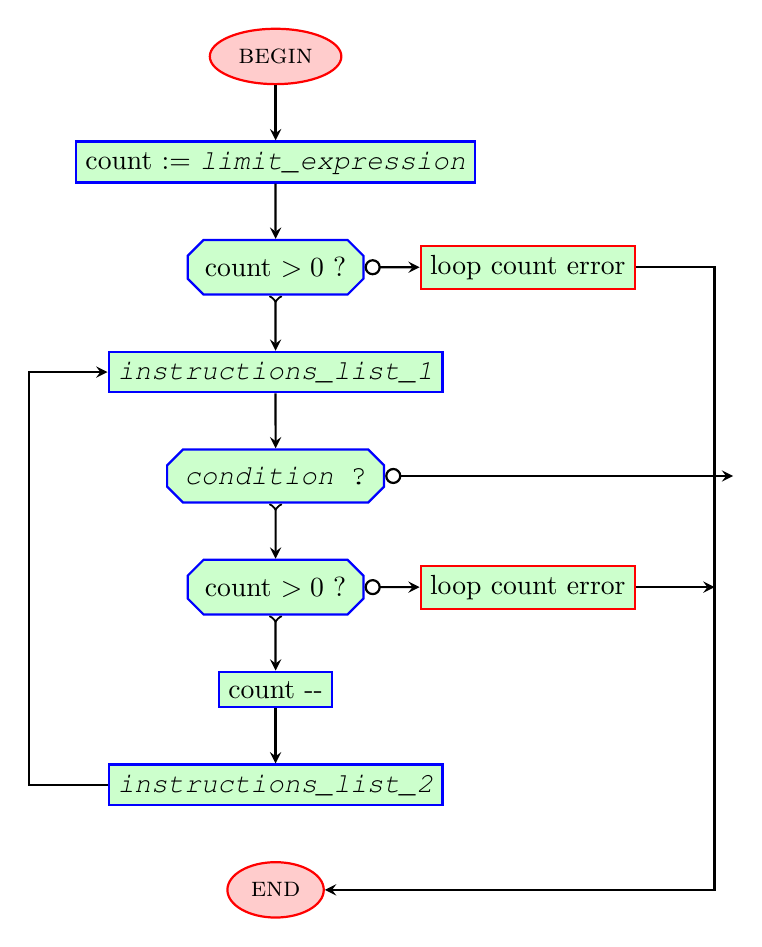
\begin{tikzpicture}[
      cloud/.style ={draw=red, thick, ellipse,fill=red!20, minimum height=2em},
      block/.style ={rectangle, draw=blue, thick, fill=green!20, align=center},
      error/.style ={rectangle, draw=red, thick, fill=green!20, align=center},
      decision/.style={chamfered rectangle, draw=blue, thick, fill=green!20},
      node distance=7mm
    ]
    \node [cloud] (start) {\textsc{begin}} ;
    \node [block] (affectationVariant) [below=of start] {count := {\tt \emph{limit_expression}}} ;
    \node [decision] (premierTest) [below=of affectationVariant] {count $> 0$ ?} ;
    \node [error] (loopVariantError) [right=of premierTest] {loop count error} ;
    \node [block] (instructions1) [below=of premierTest] {\tt \emph{instructions\_list\_1}} ;
    \node [decision] (expression) [below=of instructions1] {\tt \emph{condition} ?} ;
    \node [decision] (secondTest) [below=of expression] {count $> 0$ ?} ;
    \node [error] (loopVariantError2) [right=of secondTest] {loop count error} ;
    \node [block] (decVariant) [below=of secondTest] {count {-}{-}} ;
    \node [block] (instructions2) [below=of decVariant] {\tt \emph{instructions\_list\_2}} ;
    \node [cloud] (end) [below=of instructions2] {\textsc{end}} ;
    
    \draw [-stealth, thick] (start) -- (affectationVariant) ;
    \draw [-stealth, thick] (affectationVariant) -- (premierTest) ;
    \draw [o-stealth, thick] (premierTest) -- (loopVariantError) ;
    \draw [o-stealth, thick] (secondTest) -- (loopVariantError2) ;
    \draw [-stealth, thick] (loopVariantError.east) -- +(1, 0) |- (end.east) ;
    \draw [-stealth, thick] (loopVariantError2.east) -- +(1, 0) ;
    \draw [o-stealth, thick] (expression.east) -- +(4.42, 0) ;
    \draw [-stealth, thick] (instructions1) -- (expression) ;
    \draw [>-stealth, thick] (premierTest) -- (instructions1) ;
    \draw [>-stealth, thick] (expression) -- (secondTest) ;
    \draw [>-stealth, thick] (secondTest) -- (decVariant) ;
    \draw [-stealth, thick] (decVariant) -- (instructions2) ;
    \draw [-stealth, thick] (instructions2.west) -- +(-1, 0) |- (instructions1.west) ;
  \end{tikzpicture}
  \caption{semantics of the \emph{repeat} instruction}
  \label{fig:repeat}
\end{figure}

\end{document}  